\documentclass[12pt, a4paper]{article}
\usepackage{graphicx}
%
%Ours
\usepackage[USenglish]{babel}
\usepackage{todonotes}
\usepackage{etoolbox}
\usepackage{amsmath}
\usepackage{subfig}
\usepackage{tikz}
\usepackage{footnote}
\usepackage{amsmath}
\usepackage{float}
\usepackage{hhline}
\usepackage{cite}
\usepackage[inline]{enumitem}
\usepackage[all]{foreign}
\usepackage{nicefrac}
\usepackage[section]{placeins}
%\usepackage{showframe}
\usepackage{adjustbox}

\newcommand*{\emphColorSlide}[1]{\textcolor{ForestGreen}{\textbf{#1}}}
\newcommand*{\emphSlide}[1]{\textcolor{ForestGreen}{\textbf{#1}}}

\newcommand*{\lowEmph}[1]{\textcolor{NavyBlue}{\textbf{#1}}}
\newcommand*{\subt}{\textcolor{NavyBlue}{\textbf{<:}}}
\newcommand*{\supt}{\textcolor{NavyBlue}{\textbf{:>}}}



\newcommand{\dataflow}{data-flow}
\newcommand{\Dataflow}{Data-flow}
\newcommand{\code}[1]{\texttt{\lstinline[basicstyle=\normalsize\ttfamily,identifierstyle={\normalsize},commentstyle={\normalsize\itshape},keywordstyle={\normalsize\bfseries},ndkeywordstyle={\normalsize},stringstyle={\normalsize\ttfamily},numberstyle={\normalsize}]!#1!}}
\newcommand{\CFG}{CFG}
\newcommand{\intraj}{\emphColorSlide{\textsc{Intra}J}}
\newcommand{\intrajs}{\emphColorSlide{\textsc{IntraJ}}}
\newcommand{\intracfgs}{\emphColorSlide{\textsc{IntraCFG}}}
\newcommand{\jastaddjintraflow}{\textsc{jastaddj-intraflow}}
\newcommand{\jji}{\code{JJI}}
\newcommand{\jastadd}{\textsc{JastAdd}}
\newcommand{\extendj}{\textsc{ExtendJ}}
\newcommand{\cG}{\mathcal{G}}
\newcommand{\cV}{\mathcal{V}}
\newcommand{\cE}{\rightarrowtail}
\newcommand{\cP}{\mathcal{P}}
\newcommand{\cM}{\mathcal{M}}


\newcommand{\mSyn}{\ensuremath{\uparrow}}
\newcommand{\mInh}{\ensuremath{\downarrow}}
\newcommand{\mHOA}{\ensuremath{\rightarrow}}
\newcommand{\mColl}{\ensuremath{\square}}
\newcommand{\mCirc}{\ensuremath{\circlearrowleft}}

\newcommand{\Abase}[1]{\textcolor{ATGsym}{\mbox{\umlcode{#1}}}}
\newcommand{\Asyn}[1]{\textcolor{ATGsym}{\mbox{\mSyn{}\umlcode{#1}}}}
\newcommand{\Ainh}[1]{\textcolor{ATGsym}{\mbox{\mInh{}\umlcode{#1}}}}
\newcommand{\Ahoa}[1]{\textcolor{ATGsym}{\mbox{\mHOA{}\umlcode{#1}}}}
\newcommand{\Acoll}[1]{\textcolor{ATGsym}{\mbox{\mColl{}\umlcode{#1}}}}
\newcommand{\Acirc}[1]{\textcolor{ATGsym}{\mbox{\mCirc{}\umlcode{#1}}}}

\newcommand{\umlcode}[1]{\textrm{#1}}  % Style of code used in UML fragments
\newcommand{\astnodestyle}{\ttfamily\color{magenta}}
\newcommand{\astnode}[1]{\texttt{\textcolor{magenta}{#1}}}  % Style used for AST node types

\newcommand{\ASTUnrestricted}{AST-unrestricted}
\newcommand{\ParentFirst}{Parent-First}

\newcommand{\project}[1]{\textsc{#1}}
\newcommand{\tool}[1]{\textsc{#1}}

% can't get fbox to work reliably in the UML code, and adjustbox and nested \tikz don't work at all
%\newcommand{\dfapi}{\textsf{\setlength{\fboxsep}{0pt}\fcolorbox{blue}{white}{df-api}}}
\newcommand{\dfapi}{\textbf{\textcolor{black}{[df-api]}}}
\newcommand{\nameapi}{\textbf{\textcolor{black}{[name-api]}}}

\newcommand{\frameworkname}{\textsc{Intra}CFG}
\newcommand{\intracfg}{\textsc{\frameworkname}}

\newcommand{\node}{\mathsf{n}}
\newcommand{\Null}{\mathtt{NULL}}
\newcommand{\Notnull}{\mathtt{NOTNULL}}
\newcommand{\gen}{\mathtt{gen}}
\renewcommand{\kill}{\mathtt{kill}}

\newcommand{\In}{\mathtt{in}}
\newcommand{\Out}{\mathtt{out}}
\newcommand{\Use}{\mathtt{use}}
\newcommand{\Def}{\mathtt{def}}
\newcommand{\tf}{f_t}
\newcommand{\mCi}[1]{ { \textcolor{black!30}{\tiny \pm\text{#1}}}}%Condifdence interval

\newcommand{\CR}[1]{\textbf{[}\textcolor{blue!60!black}{\textbf{CR:} #1}\textbf{]}}
\newcommand{\Ckw}[1]{\texttt{\textbf{#1}}}
\newcommand{\auxlabel}[1]{{\scriptsize{$\textrm{\texttt{#1}}$}}}
\newcommand{\auxlabeli}[2]{{\scriptsize{$\textrm{\texttt{#2}}_{#1}$}}}
\newcommand{\auxlabelbox}[1]{\tikz[baseline=-0.7ex] \node[rectangle, minimum width=0, thin, draw, rounded corners, fill=white, inner sep=2pt, outer sep=0pt] (N) {\auxlabel{#1}};}
\newcommand{\auxlabelboxhoa}[1]{\tikz[baseline=-0.7ex] \node[rectangle, dashed,minimum width=0, thin, draw, rounded corners, fill=white, inner sep=2pt, outer sep=0pt] (N) {\auxlabel{#1}};}

%\newcommand{\auxlabelboxi}[2]{\tikz \node[rectangle, minimum width=0, thin, draw, rounded corners, fill=white] {\auxlabeli{#1}{#2}};}

\newcommand{\Prod}{::=}
\newcommand{\terminal}[1]{\textcolor{green!50!black}{\textit{#1}}}
\newcommand{\vmetavar}[1]{\textcolor{cyan!30!black}{\textsf{\textbf{#1}}}}
\newcommand{\vcode}[1]{\textsf{\textcolor{green!35!black}{{#1}}}}
\newcommand{\vterminal}[1]{\vcode{#1}}
\newcommand{\nta}[1]{\ensuremath{\textit{#1}}}
\newcommand{\tuple}[1]{\ensuremath{\langle #1 \rangle}}
\newcommand{\nt}[1]{\ensuremath{\tuple{\hspace{-0.02cm}\nta{#1}\hspace{0.02cm}}}}
\newcommand{\VB}{\ |\ }
\newcommand{\Gcomment}[1]{\textrm{\textcolor{black!50!white}{({#1})}}}
\newcommand{\sem}[1]{\ensuremath{\llbracket #1 \rrbracket}}
%\newcommand{\semNPA}[1]{\ensuremath{\sem{#1}_{\textit{NPA}}}}
\newcommand{\semNPA}[1]{\ensuremath{\sem{#1}}}

\newcommand{\listingsfontsize}{\scriptsize}

\newcommand{\NAmark}{\multicolumn{1}{c}{\textcolor{black!40!white}{-}}}
\newcommand{\NAmarkR}{\multicolumn{1}{c|}{\textcolor{black!40!white}{-}}}
\newcommand{\Tcenter}[1]{\multicolumn{1}{c}{#1}}
\newcommand{\TcenterR}[1]{\multicolumn{1}{c|}{#1}}
\newcommand{\succarrow}{\tikz[baseline=-0.7ex] \draw[succarrow, thick, -{Stealth[scale=0.9, inset=0pt, angle'=45]}] (0,0) -- (0.3,0.0);}

\colorlet{hlgreen}{green}
\colorlet{hlorange}{orange}
\colorlet{hlgreenhalf}{green!50!white}
\colorlet{hlorangehalf}{orange!50!white}
\colorlet{npagrey}{gray!10!white}

\DeclareRobustCommand{\hlgreen}[1]{{\sethlcolor{hlgreenhalf}\hl{#1}}}
\DeclareRobustCommand{\hlorange}[1]{{\sethlcolor{hlorangehalf}\hl{#1}}}

\definecolor{ATGsym}{HTML}{206010}

\definecolor{SQ}{HTML}{0080ff}
\definecolor{JJI}{HTML}{ff0080}
\definecolor{IJnonH}{HTML}{004010}
\definecolor{IJH}{HTML}{00ff20}

\definecolor{succarrow}{HTML}{4e90e2}	% adapted from RunningExample.tex

\definecolor{lightblue}{HTML}{006699}		%#006699
\definecolor{lightgreen}{HTML}{669900}		%#669900
\lstdefinelanguage{JastAdd}{
  %keyword1&2&6
  morekeywords = [1]{class, extends, private, void,new},
  %keyword3
  morekeywords = [2]{this,null}, %JASTADD keywords
  %keyword4
  morekeywords = [3]{return}, %ASTnode typess
  %keyword5
  morekeywords = [4]{},
  keywordstyle = [1]\color{lightblue},
  keywordstyle = [2]\color{lightgreen},
%  keywordstyle = [1]\bfseries,
%  keywordstyle = [2]\bfseries,
  keywordstyle = [3]\astnodestyle,
  keywordstyle = [4]\color{orange},
  sensitive = true,
  morecomment = [l]{//},
  morecomment = [s]{/*}{*/},
  morecomment = [s]{/**}{*/},
  commentstyle = \color{gray},
  morestring = [b]",
  morestring = [b]',
  stringstyle = \color{purple}
}
\lstset{
  backgroundcolor =\color{npagrey},
  basicstyle=\listingsfontsize\ttfamily,
  identifierstyle={\listingsfontsize},
  commentstyle={\listingsfontsize\itshape},
  keywordstyle={\listingsfontsize\bfseries},
  ndkeywordstyle={\listingsfontsize},
  stringstyle={\listingsfontsize\ttfamily},
  frame={tb},
  breaklines=true,
  breakatwhitespace=true, %To avoid linebreaks between \code{} and comma.
  columns=[l]{fullflexible},
  numbers=none,
  numberstyle={\listingsfontsize},
  stepnumber=1,
  mathescape,
	escapeinside     = {!}{!}, %General escape does not seem to work in lstinline/GH.
}

\makeatletter
\pgfdeclareshape{topbottombox}{
  \inheritsavedanchors[from=rectangle]
  \inheritanchorborder[from=rectangle]
  \inheritanchor[from=rectangle]{center}
  \inheritanchor[from=rectangle]{base}
  \inheritanchor[from=rectangle]{north}
  \inheritanchor[from=rectangle]{north east}
  \inheritanchor[from=rectangle]{east}
  \inheritanchor[from=rectangle]{south east}
  \inheritanchor[from=rectangle]{south}
  \inheritanchor[from=rectangle]{south west}
  \inheritanchor[from=rectangle]{west}
  \inheritanchor[from=rectangle]{north west}
  \backgroundpath{
    %  store lower right in xa/ya and upper right in xb/yb
    \southwest \pgf@xa=\pgf@x \pgf@ya=\pgf@y
    \northeast \pgf@xb=\pgf@x \pgf@yb=\pgf@y
    \pgfpathmoveto{\pgfpoint{\pgf@xa}{\pgf@ya}}
    \pgfpathlineto{\pgfpoint{\pgf@xb}{\pgf@ya}}
    \pgfpathmoveto{\pgfpoint{\pgf@xa}{\pgf@yb}}
    \pgfpathlineto{\pgfpoint{\pgf@xb}{\pgf@yb}}
 }
}
\makeatother


% Patch UML package pgf-umlcd to be able to write abstract grammar as class name.
\ExplSyntaxOn
\NewDocumentCommand{\defineclassname}{m}
 {
  \tl_set:Nn \umlcdClassName { #1 }
  \tl_set_eq:NN \umlcdClassNameString \umlcdClassName
  \tl_replace_all:Nfn \umlcdClassName { \char_generate:nn { `_ } { 8 } } { \_\kern1pt }
 }
\cs_generate_variant:Nn \tl_replace_all:Nnn { Nf }
\ExplSyntaxOff
\xpatchcmd{\classAndInterfaceCommon}
 {\def\umlcdClassName}
 {\defineclassname}
 {}{}
\xpatchcmd{\endclass}
 {(\umlcdClassName)}
 {(\umlcdClassNameString)}
 {}{\ddt}
\xpatchcmd{\endinterface}
 {(\umlcdClassName)}
 {(\umlcdClassNameString)}
 {}{\ddt}
\xpatchcmd{\endabstractclass}
 {(\umlcdClassName)}
 {(\umlcdClassNameString)}
 {}{\ddt}
\xpatchcmd{\endobject}
 {(\umlcdClassName)}
 {(\umlcdClassNameString)}
 {}{\ddt}
\xpatchcmd{\endclassAndInterfaceCommon}
 {(\umlcdClassName)}
 {(\umlcdClassNameString)}
 {}{\ddt}
\xpatchcmd{\endclassAndInterfaceCommon}
 {(\umlcdClassName)}
 {(\umlcdClassNameString)}
 {}{\ddt}
\xpatchcmd{\endclassAndInterfaceCommon}
 {(\umlcdClassName)}
 {(\umlcdClassNameString)}
 {}{\ddt}

\newbool{ANON}
%\booltrue{ANON}
\boolfalse{ANON}
\newcommand{\anon}[2]
{\ifbool{ANON}{
   #1
}{
   #2
}}


%
%
%
\begin{document}

\begin{figure}[H]
	\centering
	

\tikzset{every picture/.style={line width=0.75pt}} %set default line width to 0.75pt        

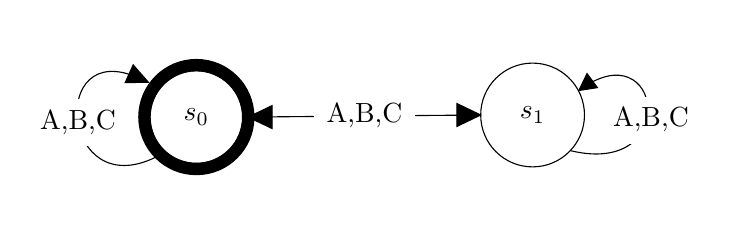
\begin{tikzpicture}[x=0.75pt,y=0.75pt,yscale=-1,xscale=1]
%uncomment if require: \path (0,300); %set diagram left start at 0, and has height of 300

%Shape: Circle [id:dp03041330611239501] 
\draw   (100,136) .. controls (100,122.19) and (111.19,111) .. (125,111) .. controls (138.81,111) and (150,122.19) .. (150,136) .. controls (150,149.81) and (138.81,161) .. (125,161) .. controls (111.19,161) and (100,149.81) .. (100,136) -- cycle ;
%Shape: Circle [id:dp06778329694496121] 
\draw   (262,135) .. controls (262,121.19) and (273.19,110) .. (287,110) .. controls (300.81,110) and (312,121.19) .. (312,135) .. controls (312,148.81) and (300.81,160) .. (287,160) .. controls (273.19,160) and (262,148.81) .. (262,135) -- cycle ;
%Straight Lines [id:da33786910107719414] 
\draw    (262,135) -- (150,136) ;


%Shape: Circle [id:dp28310457724521987] 
\draw   (102.6,136) .. controls (102.6,123.63) and (112.63,113.6) .. (125,113.6) .. controls (137.37,113.6) and (147.4,123.63) .. (147.4,136) .. controls (147.4,148.37) and (137.37,158.4) .. (125,158.4) .. controls (112.63,158.4) and (102.6,148.37) .. (102.6,136) -- cycle ;
%Shape: Circle [id:dp9488628075819832] 
\draw  [line width=4.5]  (100,136) .. controls (100,122.19) and (111.19,111) .. (125,111) .. controls (138.81,111) and (150,122.19) .. (150,136) .. controls (150,149.81) and (138.81,161) .. (125,161) .. controls (111.19,161) and (100,149.81) .. (100,136) -- cycle ;
%Curve Lines [id:da15096966683993052] 
\draw    (105.72,155.18) .. controls (59.72,178.18) and (53.3,97.2) .. (97.3,117.2) ;


%Shape: Triangle [id:dp024620734385268905] 
\draw  [fill={rgb, 255:red, 0; green, 0; blue, 0 }  ,fill opacity=1 ] (101.95,119.29) -- (90.74,119.35) -- (94.56,110.87) -- cycle ;
%Curve Lines [id:da3650058854241438] 
\draw    (309.3,123.2) .. controls (349.3,93.2) and (359.3,165.2) .. (305.3,152.2) ;


%Shape: Triangle [id:dp6528725824186807] 
\draw  [fill={rgb, 255:red, 0; green, 0; blue, 0 }  ,fill opacity=1 ] (309.3,123.2) -- (313.22,115.05) -- (318.23,121.81) -- cycle ;
%Shape: Triangle [id:dp5954374173670742] 
\draw  [fill={rgb, 255:red, 0; green, 0; blue, 0 }  ,fill opacity=1 ] (262,135) -- (250.5,140.53) -- (250.5,129.47) -- cycle ;
%Shape: Triangle [id:dp7130809704304564] 
\draw  [fill={rgb, 255:red, 0; green, 0; blue, 0 }  ,fill opacity=1 ] (150,136) -- (161.5,130.47) -- (161.5,141.53) -- cycle ;

% Text Node
\draw (125,136) node  [align=left] {$s_0$};
% Text Node
\draw (287,135) node  [align=left] {$s_1$};
% Text Node
\draw  [color={rgb, 255:red, 255; green, 255; blue, 255 }  ,draw opacity=1 ][fill={rgb, 255:red, 255; green, 255; blue, 255 }  ,fill opacity=1 ]  (182,124.5) -- (230,124.5) -- (230,146.5) -- (182,146.5) -- cycle  ;
\draw (206,135.5) node  [align=left] {A,B,C};
% Text Node
\draw  [color={rgb, 255:red, 255; green, 255; blue, 255 }  ,draw opacity=1 ][fill={rgb, 255:red, 255; green, 255; blue, 255 }  ,fill opacity=1 ]  (44,127.5) -- (92,127.5) -- (92,149.5) -- (44,149.5) -- cycle  ;
\draw (68,138.5) node  [align=left] {A,B,C};
% Text Node
\draw  [color={rgb, 255:red, 255; green, 255; blue, 255 }  ,draw opacity=1 ][fill={rgb, 255:red, 255; green, 255; blue, 255 }  ,fill opacity=1 ]  (320,126.5) -- (368,126.5) -- (368,148.5) -- (320,148.5) -- cycle  ;
\draw (344,137.5) node  [align=left] {A,B,C};


\end{tikzpicture}

	\caption{Initial State.}
\end{figure}%
\begin{align*}
s_0 &= \bra{\looking b,\looking c, \opened}\\
s_1 &= \bra{\looking{b},\looking{c},\opened,\head}
\end{align*}

\begin{figure}[H]
	\centering
	

\tikzset{every picture/.style={line width=0.75pt}} %set default line width to 0.75pt        

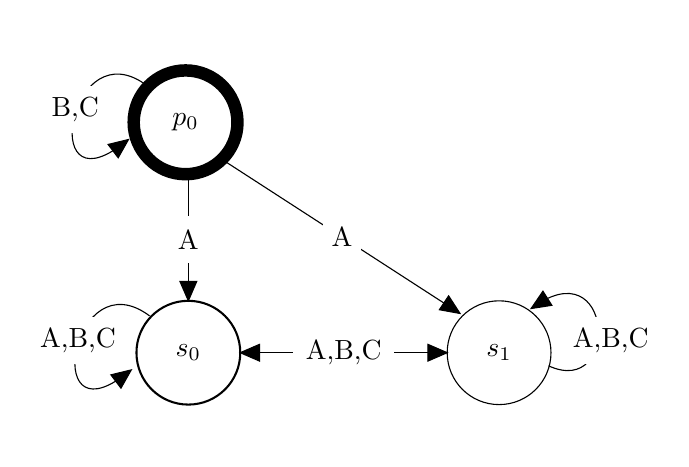
\begin{tikzpicture}[x=0.75pt,y=0.75pt,yscale=-1,xscale=1]
%uncomment if require: \path (0,300); %set diagram left start at 0, and has height of 300

%Shape: Circle [id:dp8938158972072578] 
\draw  [line width=0.75]  (105.29,143) .. controls (105.29,129.19) and (116.48,118) .. (130.29,118) .. controls (144.09,118) and (155.29,129.19) .. (155.29,143) .. controls (155.29,156.81) and (144.09,168) .. (130.29,168) .. controls (116.48,168) and (105.29,156.81) .. (105.29,143) -- cycle ;
%Shape: Circle [id:dp19780391712041556] 
\draw   (255,143) .. controls (255,129.19) and (266.19,118) .. (280,118) .. controls (293.81,118) and (305,129.19) .. (305,143) .. controls (305,156.81) and (293.81,168) .. (280,168) .. controls (266.19,168) and (255,156.81) .. (255,143) -- cycle ;
%Straight Lines [id:da018251469869151382] 
\draw    (155.29,143) -- (255,143) ;


%Shape: Triangle [id:dp4725710951486233] 
\draw  [fill={rgb, 255:red, 0; green, 0; blue, 0 }  ,fill opacity=1 ] (102.8,151.28) -- (97.82,160.08) -- (92.97,153.67) -- cycle ;
%Shape: Triangle [id:dp08394946096129607] 
\draw  [fill={rgb, 255:red, 0; green, 0; blue, 0 }  ,fill opacity=1 ] (255,143) -- (245.72,147.02) -- (245.72,138.98) -- cycle ;
%Shape: Triangle [id:dp12888926826248426] 
\draw  [fill={rgb, 255:red, 0; green, 0; blue, 0 }  ,fill opacity=1 ] (155.29,143) -- (164.56,138.98) -- (164.56,147.02) -- cycle ;
%Shape: Triangle [id:dp7536519811814515] 
\draw  [fill={rgb, 255:red, 0; green, 0; blue, 0 }  ,fill opacity=1 ] (295.43,121.72) -- (301.13,113.37) -- (305.42,120.17) -- cycle ;
%Curve Lines [id:da0862450190271058] 
\draw    (111.62,125.27) .. controls (74.82,97.67) and (59.1,184.08) .. (99.1,154.08) ;


%Curve Lines [id:da8507870813478686] 
\draw    (295.43,121.72) .. controls (335.43,91.72) and (338.63,165.32) .. (303.83,149.32) ;


%Shape: Circle [id:dp06782137726568571] 
\draw  [line width=4.5]  (103.95,32) .. controls (103.95,18.19) and (115.15,7) .. (128.95,7) .. controls (142.76,7) and (153.95,18.19) .. (153.95,32) .. controls (153.95,45.81) and (142.76,57) .. (128.95,57) .. controls (115.15,57) and (103.95,45.81) .. (103.95,32) -- cycle ;
%Shape: Triangle [id:dp8413979641210945] 
\draw  [fill={rgb, 255:red, 0; green, 0; blue, 0 }  ,fill opacity=1 ] (101.46,40.28) -- (96.49,49.08) -- (91.64,42.67) -- cycle ;
%Shape: Triangle [id:dp7368099608094223] 
\draw  [fill={rgb, 255:red, 0; green, 0; blue, 0 }  ,fill opacity=1 ] (261.18,124.1) -- (251.23,122.29) -- (255.69,115.61) -- cycle ;
%Curve Lines [id:da6315070066186073] 
\draw    (110.29,14.27) .. controls (73.49,-13.33) and (57.76,73.08) .. (97.76,43.08) ;


%Straight Lines [id:da7382395640533164] 
\draw    (130.29,59) -- (130.29,118) ;


%Straight Lines [id:da3690444677581517] 
\draw    (147.37,50.44) -- (261.18,124.1) ;


%Shape: Triangle [id:dp417855807516911] 
\draw  [fill={rgb, 255:red, 0; green, 0; blue, 0 }  ,fill opacity=1 ] (130.29,118) -- (126.27,108.72) -- (134.3,108.72) -- cycle ;

% Text Node
\draw (130.29,143) node  [align=left] {$s_0$};
% Text Node
\draw (280,143) node  [align=left] {$s_1$};
% Text Node
\draw  [color={rgb, 255:red, 255; green, 255; blue, 255 }  ,draw opacity=1 ][fill={rgb, 255:red, 255; green, 255; blue, 255 }  ,fill opacity=1 ]  (181.14,132) -- (229.14,132) -- (229.14,154) -- (181.14,154) -- cycle  ;
\draw (205.14,143) node  [align=left] {A,B,C};
% Text Node
\draw  [color={rgb, 255:red, 255; green, 255; blue, 255 }  ,draw opacity=1 ][fill={rgb, 255:red, 255; green, 255; blue, 255 }  ,fill opacity=1 ]  (53.14,126) -- (101.14,126) -- (101.14,148) -- (53.14,148) -- cycle  ;
\draw (77.14,137) node  [align=left] {A,B,C};
% Text Node
\draw  [color={rgb, 255:red, 255; green, 255; blue, 255 }  ,draw opacity=1 ][fill={rgb, 255:red, 255; green, 255; blue, 255 }  ,fill opacity=1 ]  (309.81,126) -- (357.81,126) -- (357.81,148) -- (309.81,148) -- cycle  ;
\draw (333.81,137) node  [align=left] {A,B,C};
% Text Node
\draw (128.95,32) node  [align=left] {$p_0$};
% Text Node
\draw  [color={rgb, 255:red, 255; green, 255; blue, 255 }  ,draw opacity=1 ][fill={rgb, 255:red, 255; green, 255; blue, 255 }  ,fill opacity=1 ]  (59.31,15) -- (92.31,15) -- (92.31,37) -- (59.31,37) -- cycle  ;
\draw (75.81,26) node  [align=left] {B,C};
% Text Node
\draw  [color={rgb, 255:red, 255; green, 255; blue, 255 }  ,draw opacity=1 ][fill={rgb, 255:red, 255; green, 255; blue, 255 }  ,fill opacity=1 ]  (121.29,77.5) -- (139.29,77.5) -- (139.29,99.5) -- (121.29,99.5) -- cycle  ;
\draw (130.29,88.5) node  [align=left] {A};
% Text Node
\draw  [color={rgb, 255:red, 255; green, 255; blue, 255 }  ,draw opacity=1 ][fill={rgb, 255:red, 255; green, 255; blue, 255 }  ,fill opacity=1 ]  (195.27,76.27) -- (213.27,76.27) -- (213.27,98.27) -- (195.27,98.27) -- cycle  ;
\draw (204.27,87.27) node  [align=left] {A};


\end{tikzpicture}

	\caption{State after \peek{B} where $p_0 = \bra{\looking b,\looking c, \opened}$.}
\end{figure}%


\begin{figure}[H]
	\centering
	

\tikzset{every picture/.style={line width=0.75pt}} %set default line width to 0.75pt        

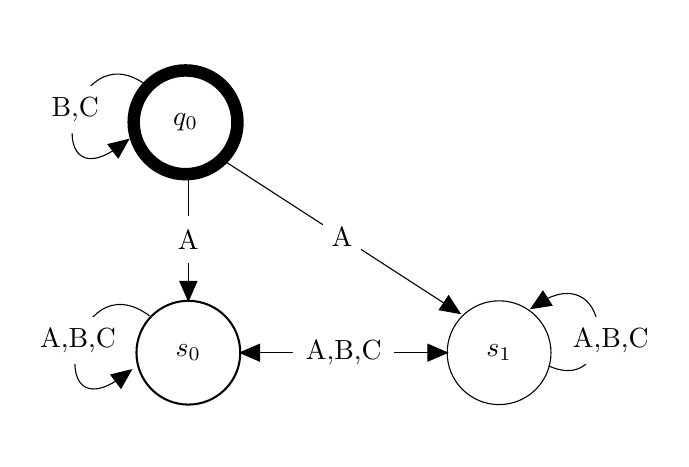
\begin{tikzpicture}[x=0.75pt,y=0.75pt,yscale=-1,xscale=1]
%uncomment if require: \path (0,300); %set diagram left start at 0, and has height of 300

%Shape: Circle [id:dp8938158972072578] 
\draw  [line width=0.75]  (105.29,143) .. controls (105.29,129.19) and (116.48,118) .. (130.29,118) .. controls (144.09,118) and (155.29,129.19) .. (155.29,143) .. controls (155.29,156.81) and (144.09,168) .. (130.29,168) .. controls (116.48,168) and (105.29,156.81) .. (105.29,143) -- cycle ;
%Shape: Circle [id:dp19780391712041556] 
\draw   (255,143) .. controls (255,129.19) and (266.19,118) .. (280,118) .. controls (293.81,118) and (305,129.19) .. (305,143) .. controls (305,156.81) and (293.81,168) .. (280,168) .. controls (266.19,168) and (255,156.81) .. (255,143) -- cycle ;
%Straight Lines [id:da018251469869151382] 
\draw    (155.29,143) -- (255,143) ;


%Shape: Triangle [id:dp4725710951486233] 
\draw  [fill={rgb, 255:red, 0; green, 0; blue, 0 }  ,fill opacity=1 ] (102.8,151.28) -- (97.82,160.08) -- (92.97,153.67) -- cycle ;
%Shape: Triangle [id:dp08394946096129607] 
\draw  [fill={rgb, 255:red, 0; green, 0; blue, 0 }  ,fill opacity=1 ] (255,143) -- (245.72,147.02) -- (245.72,138.98) -- cycle ;
%Shape: Triangle [id:dp12888926826248426] 
\draw  [fill={rgb, 255:red, 0; green, 0; blue, 0 }  ,fill opacity=1 ] (155.29,143) -- (164.56,138.98) -- (164.56,147.02) -- cycle ;
%Shape: Triangle [id:dp7536519811814515] 
\draw  [fill={rgb, 255:red, 0; green, 0; blue, 0 }  ,fill opacity=1 ] (295.43,121.72) -- (301.13,113.37) -- (305.42,120.17) -- cycle ;
%Curve Lines [id:da0862450190271058] 
\draw    (111.62,125.27) .. controls (74.82,97.67) and (59.1,184.08) .. (99.1,154.08) ;


%Curve Lines [id:da8507870813478686] 
\draw    (295.43,121.72) .. controls (335.43,91.72) and (338.63,165.32) .. (303.83,149.32) ;


%Shape: Circle [id:dp06782137726568571] 
\draw  [line width=4.5]  (103.95,32) .. controls (103.95,18.19) and (115.15,7) .. (128.95,7) .. controls (142.76,7) and (153.95,18.19) .. (153.95,32) .. controls (153.95,45.81) and (142.76,57) .. (128.95,57) .. controls (115.15,57) and (103.95,45.81) .. (103.95,32) -- cycle ;
%Shape: Triangle [id:dp8413979641210945] 
\draw  [fill={rgb, 255:red, 0; green, 0; blue, 0 }  ,fill opacity=1 ] (101.46,40.28) -- (96.49,49.08) -- (91.64,42.67) -- cycle ;
%Shape: Triangle [id:dp7368099608094223] 
\draw  [fill={rgb, 255:red, 0; green, 0; blue, 0 }  ,fill opacity=1 ] (261.18,124.1) -- (251.23,122.29) -- (255.69,115.61) -- cycle ;
%Curve Lines [id:da6315070066186073] 
\draw    (110.29,14.27) .. controls (73.49,-13.33) and (57.76,73.08) .. (97.76,43.08) ;


%Straight Lines [id:da7382395640533164] 
\draw    (130.29,59) -- (130.29,118) ;


%Straight Lines [id:da3690444677581517] 
\draw    (147.37,50.44) -- (261.18,124.1) ;


%Shape: Triangle [id:dp417855807516911] 
\draw  [fill={rgb, 255:red, 0; green, 0; blue, 0 }  ,fill opacity=1 ] (130.29,118) -- (126.27,108.72) -- (134.3,108.72) -- cycle ;

% Text Node
\draw (130.29,143) node  [align=left] {$s_0$};
% Text Node
\draw (280,143) node  [align=left] {$s_1$};
% Text Node
\draw  [color={rgb, 255:red, 255; green, 255; blue, 255 }  ,draw opacity=1 ][fill={rgb, 255:red, 255; green, 255; blue, 255 }  ,fill opacity=1 ]  (181.14,132) -- (229.14,132) -- (229.14,154) -- (181.14,154) -- cycle  ;
\draw (205.14,143) node  [align=left] {A,B,C};
% Text Node
\draw  [color={rgb, 255:red, 255; green, 255; blue, 255 }  ,draw opacity=1 ][fill={rgb, 255:red, 255; green, 255; blue, 255 }  ,fill opacity=1 ]  (53.14,126) -- (101.14,126) -- (101.14,148) -- (53.14,148) -- cycle  ;
\draw (77.14,137) node  [align=left] {A,B,C};
% Text Node
\draw  [color={rgb, 255:red, 255; green, 255; blue, 255 }  ,draw opacity=1 ][fill={rgb, 255:red, 255; green, 255; blue, 255 }  ,fill opacity=1 ]  (309.81,126) -- (357.81,126) -- (357.81,148) -- (309.81,148) -- cycle  ;
\draw (333.81,137) node  [align=left] {A,B,C};
% Text Node
\draw (128.95,32) node  [align=left] {$q_0$};
% Text Node
\draw  [color={rgb, 255:red, 255; green, 255; blue, 255 }  ,draw opacity=1 ][fill={rgb, 255:red, 255; green, 255; blue, 255 }  ,fill opacity=1 ]  (59.31,15) -- (92.31,15) -- (92.31,37) -- (59.31,37) -- cycle  ;
\draw (75.81,26) node  [align=left] {B,C};
% Text Node
\draw  [color={rgb, 255:red, 255; green, 255; blue, 255 }  ,draw opacity=1 ][fill={rgb, 255:red, 255; green, 255; blue, 255 }  ,fill opacity=1 ]  (121.29,77.5) -- (139.29,77.5) -- (139.29,99.5) -- (121.29,99.5) -- cycle  ;
\draw (130.29,88.5) node  [align=left] {A};
% Text Node
\draw  [color={rgb, 255:red, 255; green, 255; blue, 255 }  ,draw opacity=1 ][fill={rgb, 255:red, 255; green, 255; blue, 255 }  ,fill opacity=1 ]  (195.27,76.27) -- (213.27,76.27) -- (213.27,98.27) -- (195.27,98.27) -- cycle  ;
\draw (204.27,87.27) node  [align=left] {A};


\end{tikzpicture}

	\caption{State after \distract{B}{C} where $q_0 = \bra{\looking c, \opened}$.}
\end{figure}%


\begin{figure}[H]
	\centering
	

\tikzset{every picture/.style={line width=0.75pt}} %set default line width to 0.75pt        

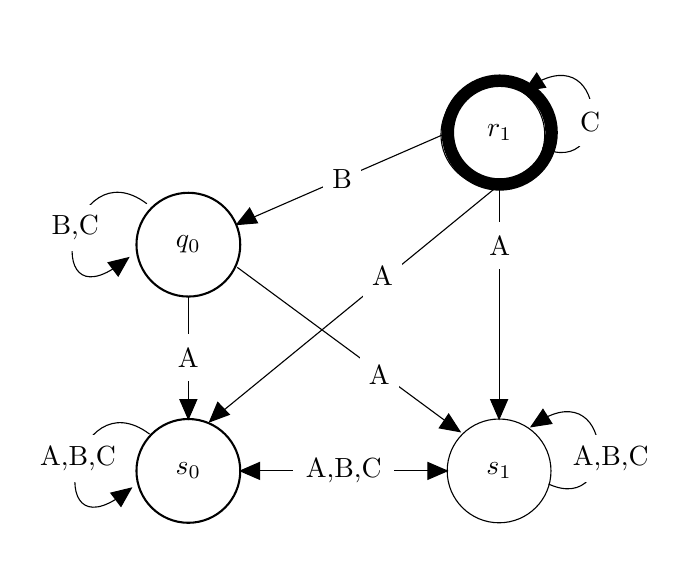
\begin{tikzpicture}[x=0.75pt,y=0.75pt,yscale=-1,xscale=1]
%uncomment if require: \path (0,300); %set diagram left start at 0, and has height of 300

%Shape: Circle [id:dp8938158972072578] 
\draw  [line width=0.75]  (135.29,223) .. controls (135.29,209.19) and (146.48,198) .. (160.29,198) .. controls (174.09,198) and (185.29,209.19) .. (185.29,223) .. controls (185.29,236.81) and (174.09,248) .. (160.29,248) .. controls (146.48,248) and (135.29,236.81) .. (135.29,223) -- cycle ;
%Shape: Circle [id:dp19780391712041556] 
\draw   (285,223) .. controls (285,209.19) and (296.19,198) .. (310,198) .. controls (323.81,198) and (335,209.19) .. (335,223) .. controls (335,236.81) and (323.81,248) .. (310,248) .. controls (296.19,248) and (285,236.81) .. (285,223) -- cycle ;
%Straight Lines [id:da018251469869151382] 
\draw    (185.29,223) -- (285,223) ;


%Shape: Triangle [id:dp4725710951486233] 
\draw  [fill={rgb, 255:red, 0; green, 0; blue, 0 }  ,fill opacity=1 ] (132.8,231.28) -- (127.82,240.08) -- (122.97,233.67) -- cycle ;
%Shape: Triangle [id:dp08394946096129607] 
\draw  [fill={rgb, 255:red, 0; green, 0; blue, 0 }  ,fill opacity=1 ] (285,223) -- (275.72,227.02) -- (275.72,218.98) -- cycle ;
%Shape: Triangle [id:dp12888926826248426] 
\draw  [fill={rgb, 255:red, 0; green, 0; blue, 0 }  ,fill opacity=1 ] (185.29,223) -- (194.56,218.98) -- (194.56,227.02) -- cycle ;
%Shape: Triangle [id:dp7536519811814515] 
\draw  [fill={rgb, 255:red, 0; green, 0; blue, 0 }  ,fill opacity=1 ] (325.43,201.72) -- (331.13,193.37) -- (335.42,200.17) -- cycle ;
%Curve Lines [id:da0862450190271058] 
\draw    (141.62,205.27) .. controls (104.82,177.67) and (89.1,264.08) .. (129.1,234.08) ;


%Curve Lines [id:da8507870813478686] 
\draw    (325.43,201.72) .. controls (365.43,171.72) and (368.63,245.32) .. (333.83,229.32) ;


%Shape: Circle [id:dp06782137726568571] 
\draw  [line width=0.75]  (135.29,114) .. controls (135.29,100.19) and (146.48,89) .. (160.29,89) .. controls (174.09,89) and (185.29,100.19) .. (185.29,114) .. controls (185.29,127.81) and (174.09,139) .. (160.29,139) .. controls (146.48,139) and (135.29,127.81) .. (135.29,114) -- cycle ;
%Shape: Triangle [id:dp8413979641210945] 
\draw  [fill={rgb, 255:red, 0; green, 0; blue, 0 }  ,fill opacity=1 ] (131.46,120.28) -- (126.49,129.08) -- (121.64,122.67) -- cycle ;
%Shape: Triangle [id:dp7368099608094223] 
\draw  [fill={rgb, 255:red, 0; green, 0; blue, 0 }  ,fill opacity=1 ] (291.18,204.1) -- (281.23,202.29) -- (285.69,195.61) -- cycle ;
%Curve Lines [id:da6315070066186073] 
\draw    (140.29,94.27) .. controls (103.49,66.67) and (87.76,153.08) .. (127.76,123.08) ;


%Straight Lines [id:da7382395640533164] 
\draw    (160.29,139) -- (160.29,198) ;


%Straight Lines [id:da3690444677581517] 
\draw    (183.87,124.94) -- (291.18,204.1) ;


%Shape: Triangle [id:dp417855807516911] 
\draw  [fill={rgb, 255:red, 0; green, 0; blue, 0 }  ,fill opacity=1 ] (160.29,198) -- (156.27,188.72) -- (164.3,188.72) -- cycle ;
%Shape: Circle [id:dp5972014220045965] 
\draw  [line width=4.5]  (285.29,60) .. controls (285.29,46.19) and (296.48,35) .. (310.29,35) .. controls (324.09,35) and (335.29,46.19) .. (335.29,60) .. controls (335.29,73.81) and (324.09,85) .. (310.29,85) .. controls (296.48,85) and (285.29,73.81) .. (285.29,60) -- cycle ;
%Shape: Triangle [id:dp4971926593318259] 
\draw  [fill={rgb, 255:red, 0; green, 0; blue, 0 }  ,fill opacity=1 ] (170.53,199.33) -- (174.44,190.01) -- (180.01,195.81) -- cycle ;
%Straight Lines [id:da46185098746714237] 
\draw    (310.29,85) -- (310.29,193.36) ;


%Straight Lines [id:da9004694794581629] 
\draw    (310.29,85) -- (170.53,199.33) ;


%Shape: Triangle [id:dp3663238051701312] 
\draw  [fill={rgb, 255:red, 0; green, 0; blue, 0 }  ,fill opacity=1 ] (310,198) -- (305.98,188.72) -- (314.02,188.72) -- cycle ;
%Shape: Circle [id:dp9462184779936802] 
\draw   (282,61) .. controls (282,47.19) and (293.19,36) .. (307,36) .. controls (320.81,36) and (332,47.19) .. (332,61) .. controls (332,74.81) and (320.81,86) .. (307,86) .. controls (293.19,86) and (282,74.81) .. (282,61) -- cycle ;
%Shape: Triangle [id:dp5745677700051097] 
\draw  [fill={rgb, 255:red, 0; green, 0; blue, 0 }  ,fill opacity=1 ] (322.43,39.72) -- (328.13,31.37) -- (332.42,38.17) -- cycle ;
%Curve Lines [id:da6922101751426857] 
\draw    (322.43,39.72) .. controls (362.43,9.72) and (365.63,83.32) .. (330.83,67.32) ;


%Straight Lines [id:da08547301161768894] 
\draw    (285.29,60) -- (183.53,104.33) ;


%Shape: Triangle [id:dp20482466216590445] 
\draw  [fill={rgb, 255:red, 0; green, 0; blue, 0 }  ,fill opacity=1 ] (183.53,104.33) -- (189.81,96.41) -- (193.6,103.49) -- cycle ;

% Text Node
\draw (160.29,223) node  [align=left] {$s_0$};
% Text Node
\draw (310,223) node  [align=left] {$s_1$};
% Text Node
\draw  [color={rgb, 255:red, 255; green, 255; blue, 255 }  ,draw opacity=1 ][fill={rgb, 255:red, 255; green, 255; blue, 255 }  ,fill opacity=1 ]  (211.14,212) -- (259.14,212) -- (259.14,234) -- (211.14,234) -- cycle  ;
\draw (235.14,223) node  [align=left] {A,B,C};
% Text Node
\draw  [color={rgb, 255:red, 255; green, 255; blue, 255 }  ,draw opacity=1 ][fill={rgb, 255:red, 255; green, 255; blue, 255 }  ,fill opacity=1 ]  (83.14,206) -- (131.14,206) -- (131.14,228) -- (83.14,228) -- cycle  ;
\draw (107.14,217) node  [align=left] {A,B,C};
% Text Node
\draw  [color={rgb, 255:red, 255; green, 255; blue, 255 }  ,draw opacity=1 ][fill={rgb, 255:red, 255; green, 255; blue, 255 }  ,fill opacity=1 ]  (339.81,206) -- (387.81,206) -- (387.81,228) -- (339.81,228) -- cycle  ;
\draw (363.81,217) node  [align=left] {A,B,C};
% Text Node
\draw (160.29,114) node  [align=left] {$q_0$};
% Text Node
\draw  [color={rgb, 255:red, 255; green, 255; blue, 255 }  ,draw opacity=1 ][fill={rgb, 255:red, 255; green, 255; blue, 255 }  ,fill opacity=1 ]  (89.31,95) -- (122.31,95) -- (122.31,117) -- (89.31,117) -- cycle  ;
\draw (105.81,106) node  [align=left] {B,C};
% Text Node
\draw  [color={rgb, 255:red, 255; green, 255; blue, 255 }  ,draw opacity=1 ][fill={rgb, 255:red, 255; green, 255; blue, 255 }  ,fill opacity=1 ]  (151.29,157.5) -- (169.29,157.5) -- (169.29,179.5) -- (151.29,179.5) -- cycle  ;
\draw (160.29,168.5) node  [align=left] {A};
% Text Node
\draw  [color={rgb, 255:red, 255; green, 255; blue, 255 }  ,draw opacity=1 ][fill={rgb, 255:red, 255; green, 255; blue, 255 }  ,fill opacity=1 ]  (243.27,165.77) -- (261.27,165.77) -- (261.27,187.77) -- (243.27,187.77) -- cycle  ;
\draw (252.27,176.77) node  [align=left] {A};
% Text Node
\draw (310.29,60) node  [align=left] {$r_1$};
% Text Node
\draw  [color={rgb, 255:red, 255; green, 255; blue, 255 }  ,draw opacity=1 ][fill={rgb, 255:red, 255; green, 255; blue, 255 }  ,fill opacity=1 ]  (301.29,103.5) -- (319.29,103.5) -- (319.29,125.5) -- (301.29,125.5) -- cycle  ;
\draw (310.29,114.5) node  [align=left] {A};
% Text Node
\draw  [color={rgb, 255:red, 255; green, 255; blue, 255 }  ,draw opacity=1 ][fill={rgb, 255:red, 255; green, 255; blue, 255 }  ,fill opacity=1 ]  (244.77,118.27) -- (262.77,118.27) -- (262.77,140.27) -- (244.77,140.27) -- cycle  ;
\draw (253.77,129.27) node  [align=left] {A};
% Text Node
\draw  [color={rgb, 255:red, 255; green, 255; blue, 255 }  ,draw opacity=1 ][fill={rgb, 255:red, 255; green, 255; blue, 255 }  ,fill opacity=1 ]  (344.31,44) -- (363.31,44) -- (363.31,66) -- (344.31,66) -- cycle  ;
\draw (353.81,55) node  [align=left] {C};
% Text Node
\draw  [color={rgb, 255:red, 255; green, 255; blue, 255 }  ,draw opacity=1 ][fill={rgb, 255:red, 255; green, 255; blue, 255 }  ,fill opacity=1 ]  (225.41,71.17) -- (243.41,71.17) -- (243.41,93.17) -- (225.41,93.17) -- cycle  ;
\draw (234.41,82.17) node  [align=left] {B};


\end{tikzpicture}

	\caption{State after \flip{C} where $r_1 = \bra{\looking c, \opened, \head}$.}
\end{figure}%


\begin{figure}[H]
	\centering
	\tikzset{every picture/.style={line width=0.75pt}} %set default line width to 0.75pt        

\trimbox{0cm 0cm 0cm 1.8cm}{ 
	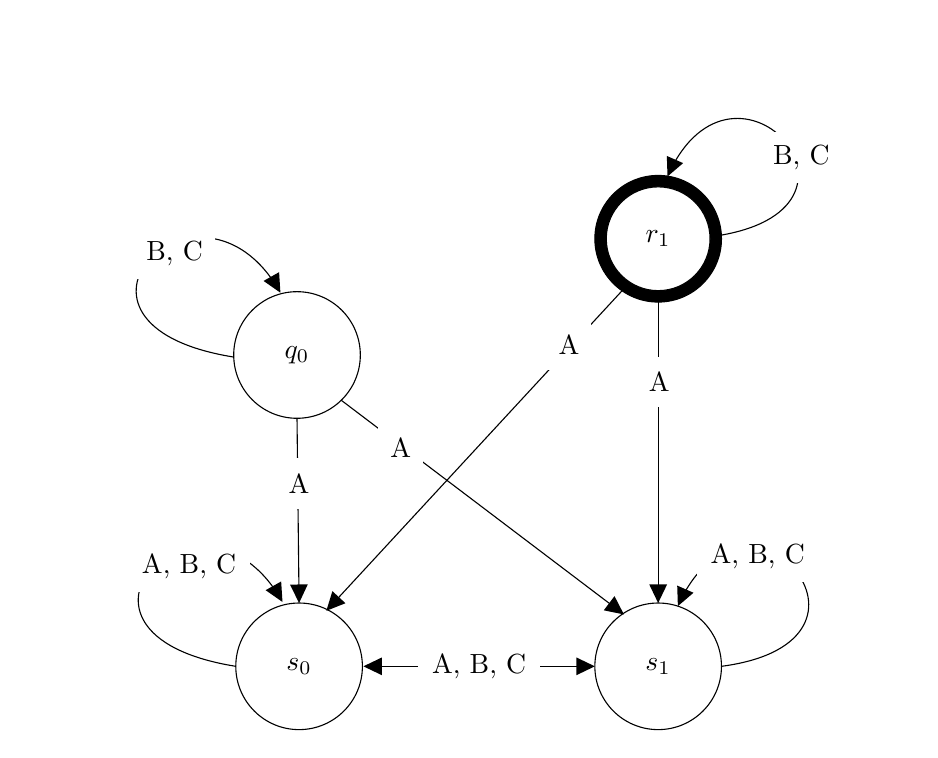
\begin{tikzpicture}[x=0.75pt,y=0.75pt,yscale=-1,xscale=1]
	%uncomment if require: \path (0,369); %set diagram left start at 0, and has height of 369
	
	%Shape: Circle [id:dp4758801382807807] 
	\draw   (93.5,322) .. controls (93.5,305.16) and (107.16,291.5) .. (124,291.5) .. controls (140.84,291.5) and (154.5,305.16) .. (154.5,322) .. controls (154.5,338.84) and (140.84,352.5) .. (124,352.5) .. controls (107.16,352.5) and (93.5,338.84) .. (93.5,322) -- cycle ;
	%Shape: Circle [id:dp5495909764900969] 
	\draw   (266.5,322) .. controls (266.5,305.16) and (280.16,291.5) .. (297,291.5) .. controls (313.84,291.5) and (327.5,305.16) .. (327.5,322) .. controls (327.5,338.84) and (313.84,352.5) .. (297,352.5) .. controls (280.16,352.5) and (266.5,338.84) .. (266.5,322) -- cycle ;
	%Straight Lines [id:da0065340714279329415] 
	\draw    (157,322) -- (264.5,322) ;
	\draw [shift={(266.5,322)}, rotate = 180] [fill={rgb, 255:red, 0; green, 0; blue, 0 }  ][line width=0.75]  [draw opacity=0] (8.93,-4.29) -- (0,0) -- (8.93,4.29) -- cycle    ;
	\draw [shift={(155,322)}, rotate = 0] [fill={rgb, 255:red, 0; green, 0; blue, 0 }  ][line width=0.75]  [draw opacity=0] (8.93,-4.29) -- (0,0) -- (8.93,4.29) -- cycle    ;
	%Curve Lines [id:da8764232980193448] 
	\draw    (93.5,322) .. controls (-5.5,306.08) and (76.67,223.33) .. (115.42,289.98) ;
	\draw [shift={(116,291)}, rotate = 240.66] [fill={rgb, 255:red, 0; green, 0; blue, 0 }  ][line width=0.75]  [draw opacity=0] (8.93,-4.29) -- (0,0) -- (8.93,4.29) -- cycle    ;
	
	%Curve Lines [id:da9911776319478228] 
	\draw    (327.5,322) .. controls (417.91,310.08) and (339.16,221.57) .. (306.98,291.93) ;
	\draw [shift={(306.5,293)}, rotate = 293.78] [fill={rgb, 255:red, 0; green, 0; blue, 0 }  ][line width=0.75]  [draw opacity=0] (8.93,-4.29) -- (0,0) -- (8.93,4.29) -- cycle    ;
	
	%Shape: Circle [id:dp7209538961655225] 
	\draw  [fill={rgb, 255:red, 0; green, 0; blue, 0 }  ,fill opacity=1 ] (266.5,116) .. controls (266.5,99.16) and (280.16,85.5) .. (297,85.5) .. controls (313.84,85.5) and (327.5,99.16) .. (327.5,116) .. controls (327.5,132.84) and (313.84,146.5) .. (297,146.5) .. controls (280.16,146.5) and (266.5,132.84) .. (266.5,116) -- cycle ;
	%Shape: Circle [id:dp27685421107424146] 
	\draw   (92.5,172) .. controls (92.5,155.16) and (106.16,141.5) .. (123,141.5) .. controls (139.84,141.5) and (153.5,155.16) .. (153.5,172) .. controls (153.5,188.84) and (139.84,202.5) .. (123,202.5) .. controls (106.16,202.5) and (92.5,188.84) .. (92.5,172) -- cycle ;
	%Shape: Circle [id:dp22158231372598314] 
	\draw  [fill={rgb, 255:red, 255; green, 255; blue, 255 }  ,fill opacity=1 ] (272,116) .. controls (272,102.19) and (283.19,91) .. (297,91) .. controls (310.81,91) and (322,102.19) .. (322,116) .. controls (322,129.81) and (310.81,141) .. (297,141) .. controls (283.19,141) and (272,129.81) .. (272,116) -- cycle ;
	%Straight Lines [id:da40013428570885556] 
	\draw    (144.3,193.8) -- (278.91,295.79) ;
	\draw [shift={(280.5,297)}, rotate = 217.15] [fill={rgb, 255:red, 0; green, 0; blue, 0 }  ][line width=0.75]  [draw opacity=0] (8.93,-4.29) -- (0,0) -- (8.93,4.29) -- cycle    ;
	
	%Straight Lines [id:da31319417430186725] 
	\draw    (281.5,139) -- (138.48,293.78) ;
	\draw [shift={(137.13,295.25)}, rotate = 312.74] [fill={rgb, 255:red, 0; green, 0; blue, 0 }  ][line width=0.75]  [draw opacity=0] (8.93,-4.29) -- (0,0) -- (8.93,4.29) -- cycle    ;
	
	%Straight Lines [id:da24005875384214737] 
	\draw    (123,202.5) -- (123.98,289.5) ;
	\draw [shift={(124,291.5)}, rotate = 269.36] [fill={rgb, 255:red, 0; green, 0; blue, 0 }  ][line width=0.75]  [draw opacity=0] (8.93,-4.29) -- (0,0) -- (8.93,4.29) -- cycle    ;
	
	%Straight Lines [id:da7741558521862318] 
	\draw    (297,146.5) -- (297,289.5) ;
	\draw [shift={(297,291.5)}, rotate = 270] [fill={rgb, 255:red, 0; green, 0; blue, 0 }  ][line width=0.75]  [draw opacity=0] (8.93,-4.29) -- (0,0) -- (8.93,4.29) -- cycle    ;
	
	%Shape: Circle [id:dp41523883310129905] 
	%\draw   (133.5,78) .. controls (133.5,61.16) and (147.16,47.5) .. (164,47.5) .. controls (180.84,47.5) and (194.5,61.16) .. (194.5,78) .. controls (194.5,94.84) and (180.84,108.5) .. (164,108.5) .. controls (147.16,108.5) and (133.5,94.84) .. (133.5,78) -- cycle ;
	%Curve Lines [id:da8202719280397651] 
	%\draw    (194.5,78) .. controls (284.91,66.08) and (206.16,-22.43) .. (173.98,47.93) ;
	%\draw [shift={(173.5,49)}, rotate = 293.78] [fill={rgb, 255:red, 0; green, 0; blue, 0 }  ][line width=0.75]  [draw opacity=0] (8.93,-4.29) -- (0,0) -- (8.93,4.29) -- cycle    ;
	
	%Curve Lines [id:da5631597181878643] 
	\draw    (322.5,115) .. controls (412.91,103.08) and (334.16,14.57) .. (301.98,84.93) ;
	\draw [shift={(301.5,86)}, rotate = 293.78] [fill={rgb, 255:red, 0; green, 0; blue, 0 }  ][line width=0.75]  [draw opacity=0] (8.93,-4.29) -- (0,0) -- (8.93,4.29) -- cycle    ;
	
	%Curve Lines [id:da7961284231370371] 
	\draw    (92.5,173) .. controls (-6.5,157.08) and (75.67,74.33) .. (114.42,140.98) ;
	\draw [shift={(115,142)}, rotate = 240.66] [fill={rgb, 255:red, 0; green, 0; blue, 0 }  ][line width=0.75]  [draw opacity=0] (8.93,-4.29) -- (0,0) -- (8.93,4.29) -- cycle    ;
	
	%Straight Lines [id:da052907042750716116] 
	%\draw    (177.5,105) -- (279.55,295.24) ;
	%\draw [shift={(280.5,297)}, rotate = 241.79] [fill={rgb, 255:red, 0; green, 0; blue, 0 }  ][line width=0.75]  [draw opacity=0] (8.93,-4.29) -- (0,0) -- (8.93,4.29) -- cycle    ;
	
	%Curve Lines [id:da9891597123428996] 
	%\draw    (95.16,339.5) .. controls (-58.51,370.39) and (40.01,-87.28) .. (140.5,56) ;
	
	%\draw [shift={(97.5,339)}, rotate = 167.09] [fill={rgb, 255:red, 0; green, 0; blue, 0 }  ][line width=0.75]  [draw opacity=0] (8.93,-4.29) -- (0,0) -- (8.93,4.29) -- cycle    ;
	
	% Text Node
	\draw  [color={rgb, 255:red, 255; green, 255; blue, 255 }  ,draw opacity=1 ][fill={rgb, 255:red, 255; green, 255; blue, 255 }  ,fill opacity=1 ]  (181.75,310) -- (239.75,310) -- (239.75,334) -- (181.75,334) -- cycle  ;
	\draw (210.75,322) node   {\agent A, \agent B, \agent C};
	% Text Node
	\draw (124,322) node   {$\defemph  s_{0}$};
	% Text Node
	\draw (297,322) node   {$\defemph  s_{1}$};
	% Text Node
	\draw  [color={rgb, 255:red, 255; green, 255; blue, 255 }  ,draw opacity=1 ][fill={rgb, 255:red, 255; green, 255; blue, 255 }  ,fill opacity=1 ]  (42,262) -- (100,262) -- (100,286) -- (42,286) -- cycle  ;
	\draw (71,274) node   {\agent A, \agent B, \agent C};
	% Text Node
	\draw  [color={rgb, 255:red, 255; green, 255; blue, 255 }  ,draw opacity=1 ][fill={rgb, 255:red, 255; green, 255; blue, 255 }  ,fill opacity=1 ]  (316,257) -- (374,257) -- (374,281) -- (316,281) -- cycle  ;
	\draw (345,269) node   {\agent A, \agent B, \agent C};
	% Text Node
	\draw (297,116) node   {$\defemph   r_{1}$};
	% Text Node
	\draw (123,172) node   {$\defemph  q_{0}$};
	% Text Node
	%\draw (164,78) node   {$\defemph  r_{1}$};
	% Text Node
	%\draw  [color={rgb, 255:red, 255; green, 255; blue, 255 }  ,draw opacity=1 ][fill={rgb, 255:red, 255; green, 255; blue, 255 }  ,fill opacity=1 ]  (213,27) -- (251,27) -- (251,51) -- (213,51) -- cycle  ;
	%\draw (232,39) node   {\agent B, \agent C};
	% Text Node
	\draw  [color={rgb, 255:red, 255; green, 255; blue, 255 }  ,draw opacity=1 ][fill={rgb, 255:red, 255; green, 255; blue, 255 }  ,fill opacity=1 ]  (243.5,155) -- (264.5,155) -- (264.5,179) -- (243.5,179) -- cycle  ;
	\draw (254,167) node   {\agent A};
	% Text Node
	\draw  [color={rgb, 255:red, 255; green, 255; blue, 255 }  ,draw opacity=1 ][fill={rgb, 255:red, 255; green, 255; blue, 255 }  ,fill opacity=1 ]  (287,173) -- (308,173) -- (308,197) -- (287,197) -- cycle  ;
	\draw (297.5,185) node   {\agent A};
	% Text Node
	%\draw  [color={rgb, 255:red, 255; green, 255; blue, 255 }  ,draw opacity=1 ][fill={rgb, 255:red, 255; green, 255; blue, 255 }  ,fill opacity=1 ]  (194.5,139) -- (215.5,139) -- (215.5,163) -- (194.5,163) -- cycle  ;
	%\draw (205,151) node   {\agent A};
	% Text Node
	\draw  [color={rgb, 255:red, 255; green, 255; blue, 255 }  ,draw opacity=1 ][fill={rgb, 255:red, 255; green, 255; blue, 255 }  ,fill opacity=1 ]  (113.5,222) -- (134.5,222) -- (134.5,246) -- (113.5,246) -- cycle  ;
	\draw (124,234) node   {\agent A};
	% Text Node
	\draw  [color={rgb, 255:red, 255; green, 255; blue, 255 }  ,draw opacity=1 ][fill={rgb, 255:red, 255; green, 255; blue, 255 }  ,fill opacity=1 ]  (162.5,205) -- (183.5,205) -- (183.5,229) -- (162.5,229) -- cycle  ;
	\draw (173,217) node   {\agent A};
	% Text Node
	\draw  [color={rgb, 255:red, 255; green, 255; blue, 255 }  ,draw opacity=1 ][fill={rgb, 255:red, 255; green, 255; blue, 255 }  ,fill opacity=1 ]  (347,65) -- (385,65) -- (385,89) -- (347,89) -- cycle  ;
	\draw (366,77) node   {\agent B, \agent C};
	% Text Node
	\draw  [color={rgb, 255:red, 255; green, 255; blue, 255 }  ,draw opacity=1 ][fill={rgb, 255:red, 255; green, 255; blue, 255 }  ,fill opacity=1 ]  (45,111) -- (83,111) -- (83,135) -- (45,135) -- cycle  ;
	\draw (64,123) node   {\agent B, \agent C};
	% Text Node
	%\draw  [color={rgb, 255:red, 255; green, 255; blue, 255 }  ,draw opacity=1 ][fill={rgb, 255:red, 255; green, 255; blue, 255 }  ,fill opacity=1 ]  (46.5,48) -- (67.5,48) -- (67.5,72) -- (46.5,72) -- cycle  ;
	%\draw (57,60) node   {\agent A};
	
	
	\end{tikzpicture}
}
	\caption{State after \tell{B}{c}.}
\end{figure}%

\end{document}
